\documentclass[10pt,twocolumn]{article}
\usepackage{bm}
\usepackage[]{graphicx}
\usepackage[margin=1in]{geometry}
\usepackage[]{hyperref}

\begin{document}

\title{Mini-project \#1}
\author{Casper Liu, Eric Quinn, Howard Huang}
\maketitle

Data set for part 2: \url{https://raw.githubusercontent.com/imcpr/linear_regression_project/master/reddit_full_data.csv}

\section{Part 1}
\subsection{Using Gradient Descent}

\subsection{Using the Matrix Equation}

Given training examples in the form of a matrix $\bm X$ and $\bm Y$, where $\bm X$ contains the features and $\bm Y$ contains the expected output, there is a closed form solution for finding a weight vector $\bm w$ such that $\bm X \bm w \approx Y$.
This vector can be computed as follows:
\[\bm w = (\bm X^T \bm X)^{-1}\bm X^T Y\]

A problem encountered here is that the matrix $(\bm X^T \bm X)$ is very close to being singular, which led to inaccuracies in inverse, and thus the resulting weight vector.
With the use of ridge regression instead, not only does it make the resulting vector non-singular, it also penalizes the use of large weights, so the weights are kept smaller, and (by Occam's Razor) would likely generalize better.

\[\bm w = (\bm X^T \bm X + \lambda \bm I)^{-1}\bm X^T Y\]

The data was used as is without any preprocessing, although the error rate may have been lower if that were not the case.

The only hyperparameters in this case is $\lambda$.
This was chosen by comparing various values ranging from $10^{-10}$ to $10^{10}$, computing the weights with that $\lambda$ and the training set, and checking the mean squared error on the validation set (See figure \ref{fig:ecurve1-lambda}).
This ensures that the chosen $\lambda$ works well in generalizing to unseen data.
The training set chosen for this procedure was a uniformly random subset of $80\%$ of the available data, and the rest was split evenly between the validation and test set.

\begin{figure}[htpb]
	\centering
	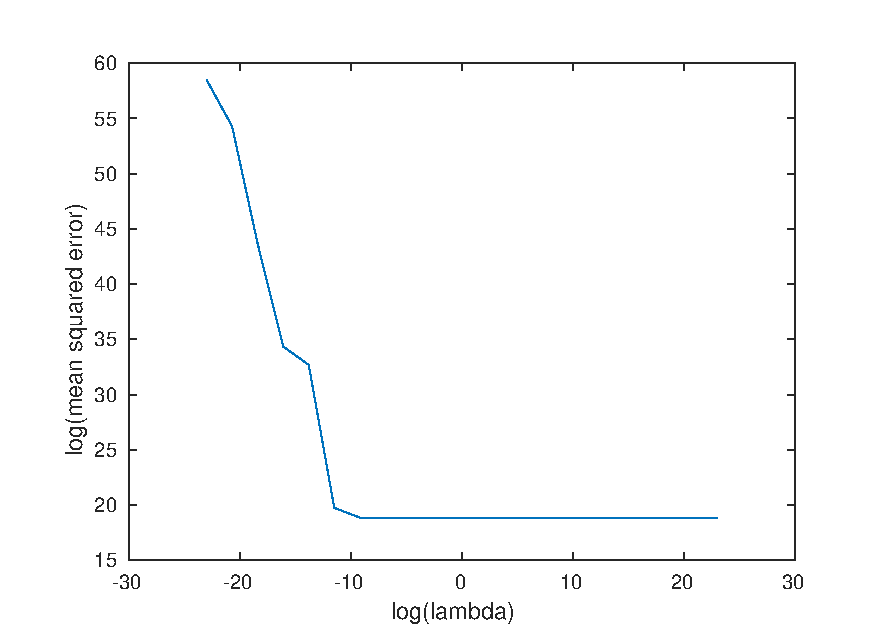
\includegraphics[width=0.5\textwidth]{part1-error-curve}
	\caption{Error curve as a function of $\lambda$}
	\label{fig:ecurve1-lambda}
\end{figure}

\subsubsection{Results}

The optimal $\lambda$ was found to be $0.01$.
This was used along with the training and validation set together to compute the weight vector.
The test set was then used to check the error of the predictions.
Averaged over $30$ runs, the average mean squared error of the testing and training set were both approximately $1.3\times 10^8$.

\subsubsection{Analysis}

A mean squared error of $1.3\times 10^8$ means that the average difference between the actual number of shares and the predicted number of shares is $\sqrt{1.3\times 10^8} = 1.1\times 10^4$.
The least squares error function applied to linear regression is convex, and has a closed form solution which returns the global optimum.
Additionally, the error is equally high both on the training set and on the test set, so it is not due to overfitting.
Therefore, the most likely explanation for this error is the high bias in the model, due to the restriction to linear models and being unable to recode features.

\section{Part 2}

\subsection{Topic Choice}
Reddit.com is a very popular website, 34th in popularity worldwide ("Reddit.com Site Overview"), which means that results relating to the site relate to many people worldwide and are worthwhile studying. In addition, submissions to the site are reasonably catalogued and split into subforums allowing for cross reference between them. The posts have a "karma score," which defines how far up on the site they will be pushed for people to view.

We have chosen data from four specific subforums because they are all popular on the website, leading to a better distribution of the resulting scores. In addition, these subforums only allow text posts, which keeps all the content constrained to just this one website. It also means that all the content of the post is available within reddit.com itself.

\subsection{Scraping techniques}
In order to collect the posts, the authors used a python scraper to browse through the "new" pages of the subforums in order and collect the links to all of the posts. We then used these links to access the permanent link to each post, which can be used to collect the actual information about the submission, not just the metadata that appears on the search page.

The authors used the Python Reddit API Wrapper (Boe) to access reddit.com in order to collect data about each submission to the four chosen subforums of the main website. This API scrapes the information about the post when given the permanent link to a submission.

We decided to only use posts that are at least two days old, at which point the submission will have fallen off the main pages for most users and the karma score should change less. This means that the data we are using is to predict the final score of a post before publishing or just after, without regard for how well it does in the first few minutes of its time on the website proper.

\subsection{Feature Selection}
\begin{verbatim}
0: num words in title
1: num words in text
2: time_of_day
3: time_of_day_squared
4: day0
5: day1
6: day2
7: day3
8: day4
9: day5
10: day6
11: sub_reddit_0 (change_my_view)
12: sub_reddit_1 (relationships)
13: sub_reddit_2 (self)
14: sub_reddit_3 (tifu)
15: sentiment_analysis
16: liberal
17: libertarian
18: conservative
19: green
20-69: top 50 words
70: upvotes
\end{verbatim}

\begin{itemize}
	\item 4-10:
		A sparse vector representing the day of the week when the contents were posted.
		The feature corresponding to the posting day has a value of $1$, and the rest are $0$.
	\item 11-14:
		A sparse vector representing the subreddit to which the contents were posted.
		The feature corresponding to the post's subreddit has a value of $1$, and the rest are $0$.
	\item 20-69:
		The top $50$ words were found by aggregating the text from every reddit post in the data set and extracting $50$ most common words, excluding stop words.
\end{itemize}

\subsection{Challenges}
Karma is not necessarily static in the time frame used.

People can raise or lower the score of a post, so it is not as simple as the number of people that see a post. This is clear in some of the data that has many comments but a score of 0, indicating it was very controversial but not agreed with enough to become popular.

Karma is hard to predict because when something becomes more popular, even more people will see it, it can grow exponentially. Posts vary substantially in popularity based on the first few minutes of their time on Reddit.com. If they gain popularity at the start, then they will appear to more people and grow in popularity even more. This is doubled by the fact that old posts will not show up to people browsing the website in the normal manner, so an old post is unlikely to be found and increase in popularity later.

Reddit makes it difficult to collect posts over a long time frame because their API does not allow collecting all posts in a given date range. The "new" page that was used for scraping only collects the most recent thousand posts or so, which makes collecting a large sample size difficult. it is possible but more difficult to get older posts than that.

\subsection{Results}

Using the same procedure as part 1, the optimal value of $\lambda$ was found to be $10^{-4}$ (See error curve in figure \ref{fig:ecurve2-lambda}).
The mean squares error was on both the training and test set were $5.6\times 10^{4}$.
The number of upvotes in the training examples range from a single upvote, up to $843300$.

\begin{figure}[htpb]
	\centering
	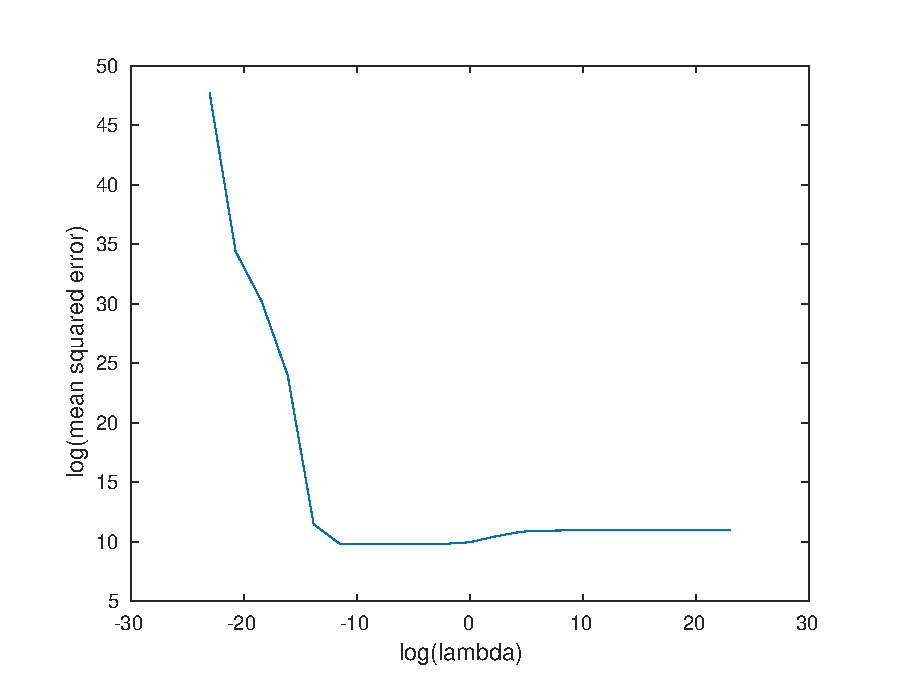
\includegraphics[width=0.5\textwidth]{part2-error-curve}
	\caption{Error curve as a function of $\lambda$}
	\label{fig:ecurve2-lambda}
\end{figure}

We hereby state that all the work presented in this report is that of the authors.
\end{document}
